\documentclass[
11pt, % Set the default font size, options include: 8pt, 9pt, 10pt, 11pt, 12pt, 14pt, 17pt, 20pt
%t, % Uncomment to vertically align all slide content to the top of the slide, rather than the default centered
%aspectratio=169, % Uncomment to set the aspect ratio to a 16:9 ratio which matches the aspect ratio of 1080p and 4K screens and projectors
]{beamer}

\graphicspath{{Images/}{./}} % Specifies where to look for included images (trailing slash required)

\usepackage{todonotes}
\usepackage{graphicx}
\usepackage{xcolor}
\usepackage{subfig}
%%\usepackage[noend]{algpseudocode}

%
%\usepackage{algorithm}
%\usepackage{algorithmic}
\usepackage{algorithm}
\usepackage{algpseudocode}
\usepackage{blkarray}
\usepackage{amsmath}
\usepackage{xspace}
\usepackage{float}


\usepackage{tikz}
\usetikzlibrary{matrix, decorations, patterns, positioning, shapes, calc, intersections, arrows, fit}

\usetikzlibrary{patterns}
\usetikzlibrary{fit,calc,positioning,decorations.pathreplacing,matrix,3d, hobby}

\usepackage{booktabs} % Allows the use of \toprule, \midrule and \bottomrule for better rules in tables
\usepackage{bm}
\usepackage{multirow}
\usepackage{ragged2e}


\newcommand{\brown}[1]{{\color{brown} #1 }}

%% Colors from https://latexcolor.com/
\definecolor{pastelviolet}{rgb}{0.8, 0.6, 0.79}
\definecolor{babyblueeyes}{rgb}{0.63, 0.79, 0.95}
\definecolor{pastelyellow}{rgb}{0.99, 0.99, 0.59}
\definecolor{pastelgreen}{rgb}{0.47, 0.87, 0.47}
\definecolor{pastelred}{rgb}{1.0, 0.41, 0.38}
\colorlet{patternblue}{blue!60}



%%\newcommand{\tensorcolor}{patternblue}
\newcommand{\tensorcolor}{cyan}


\colorlet{darkred}{red!80!black}
\colorlet{darkblue}{blue!80!black}
\newcommand<>{\darkred}[1]{{\color{darkred}{#1}}}
\newcommand<>{\darkblue}[1]{{\color#2{blue!50!black!100}{#1}}}

\newcommand{\A}{\mathbf{A}}
\newcommand{\B}{\mathbf{B}}
\newcommand{\CC}{\mathbf{C}}
%\newcommand{\Real}{\mathbb{R}}
%\newcommand{\vc}[1]{\bm{#1}}

\usetheme{Madrid}

%\newcommand{\Tra}{{\sf T}} 


%\newcommand{\Ms}[2]{\mathbf{#1}^{(#2)}} 
%\newcommand{\M}[1]{\mathbf{#1}} 
%\newcommand{\Mb}[2]{\mathbf{#1}_{#2}} 
%\newcommand{\Mbs}[3]{\mathbf{#1}_{#2}^{(#3)}} 

%\usepackage{enumitem}

%% ------------------------------------------------------------
%% PACKAGES
%% ------------------------------------------------------------

%% For \circledast
\usepackage{amssymb,amsfonts,amsmath}

%% For \mathscr
\usepackage[mathscr]{eucal}

%% For \llbracket and \rrbracket, \varoast, \varoslash
\usepackage{stmaryrd}

%% For \boldsymbol
\usepackage{amsbsy}

%% For \bm (bold math)
\usepackage{bm}

%% For \set, \Set
\usepackage{braket}

%% ------------------------------------------------------------
%% MACROS
%% ------------------------------------------------------------


%% --- Extras ---
% Transpose
\newcommand{\Tra}{{\sf T}} 
\newcommand{\parens}[1]{(#1)}
\newcommand{\Parens}[1]{\left(#1\right)}
\newcommand{\dsquare}[1]{\llbracket #1 \rrbracket}
\newcommand{\Dsquare}[1]{\left\llbracket #1 \right\rrbracket}
\newcommand{\curly}[1]{\{ #1 \}}
\newcommand{\Curly}[1]{\left\{ #1 \right\}}
\newcommand{\Real}{\mathbb{R}}
\newcommand{\qtext}[1]{\quad\text{#1}\quad}

%% --- Vectors ---
% vector
\newcommand{\V}[2][]{{\bm{#1\mathbf{\MakeLowercase{#2}}}}} 
% element of vector
\newcommand{\VE}[3][]{#1{\MakeLowercase{#2}}_{#3}} 
% vector in series
\newcommand{\Vn}[3][]{{\bm{#1\mathbf{\MakeLowercase{#2}}}}^{(#3)}} 
% transposed vector in series
\newcommand{\VnTra}[3][]{{\bm{#1\mathbf{\MakeLowercase{#2}}}}^{(#3)\Tra}} 
% element of vector in series
\newcommand{\VnE}[4][]{#1{\MakeLowercase{#2}}^{(#3)}_{#4}} 

%% --- Matrices ---
% matrix
\newcommand{\M}[2][]{{\bm{#1\mathbf{\MakeUppercase{#2}}}}} 
% matrix in series
\newcommand{\Mn}[3][]{{\bm{#1\mathbf{\MakeUppercase{#2}}}}^{(#3)}} 
% transposed matrix in series 
\newcommand{\MnTra}[4][]{{\bm{#1\mathbf{\MakeUppercase{#2}}}}^{(#3)\Tra}} 
% matrix column
\newcommand{\MC}[3][]{\V[#1]{#2}_{#3}} 
% column of matrix in series
\newcommand{\MnC}[4][]{\Vn[#1]{#2}{#3}_{#4}} 
% transposed column of matrix in series
\newcommand{\MnCTra}[4][]{\VnTra[#1]{#2}{#3}_{#4}} 
% matrix element
\newcommand{\ME}[3][]{#1{\MakeLowercase{#2}}_{#3}} 
% element of matrix in series
\newcommand{\MnE}[4][]{#1{\MakeLowercase{#2}}^{(#3)}_{#4}} 

%% --- Tensors ---
% tensor
\newcommand{\T}[2][]{\boldsymbol{#1\mathscr{\MakeUppercase{#2}}}} 
% tensor slide
\newcommand{\TS}[3][]{\M[#1]{#2}_{#3}}
% tensor element
\newcommand{\TE}[3][]{#1{\MakeLowercase{#2}}_{#3}}
% matriczied tensor
\newcommand{\Mz}[3][]{\M[#1]{#2}_{(#3)}}

%% --- Operators ---
% outer product
\newcommand{\Oprod}{\circ} 
% Kronecker product
\newcommand{\Kron}{\otimes} 
% Khatri-Rao product
\newcommand{\Khat}{\odot} 
% Hadamard (elementwise multiply)
\newcommand{\Hada}{\ast} 
\newcommand{\BigHada}{\mathop{\mbox{\fontsize{18}{19}\selectfont $\circledast$}}} 
% Elementwise divide
\newcommand{\Divi}{\varoslash}




\hypersetup{linkcolor=blue}

%----------------------------------------------------------------------------------------
%	PRESENTATION INFORMATION
%----------------------------------------------------------------------------------------

\title[MTTKRP]{Matricized tensor times Khatri-Rao product computation} % The short title in the optional parameter appears at the bottom of every slide, the full title in the main parameter is only on the title page

%\subtitle{Optional Subtitle} % Presentation subtitle, remove this command if a subtitle isn't required

\author[Suraj Kumar]{Suraj Kumar} % Presenter name(s), the optional parameter can contain a shortened version to appear on the bottom of every slide, while the main parameter will appear on the title slide

\institute[Inria \& ENS Lyon]{Inria \& ENS Lyon \\ \smallskip Email:\textit{suraj.kumar@inria.fr}} % Your institution, the optional parameter can be used for the institution shorthand and will appear on the bottom of every slide after author names, while the required parameter is used on the title slide and can include your email address or additional information on separate lines

\date[CR12]{CR12: October 2023\\ \smallskip\small https://surakuma.github.io/courses/daamtc.html} % Presentation date or conference/meeting name, the optional parameter can contain a shortened version to appear on the bottom of every slide, while the required parameter value is output to the title slide

%----------------------------------------------------------------------------------------

\begin{document}
	
	%----------------------------------------------------------------------------------------
	%	TITLE SLIDE
	%----------------------------------------------------------------------------------------
	
	\begin{frame}
		\titlepage % Output the title slide, automatically created using the text entered in the PRESENTATION INFORMATION block above
	\end{frame}

\begin{frame}{Loomis-Whitney inequality}
	\small
\begin{itemize}
	\item Relates volume of a $d$-dimensional object with its all $d-1$ dimensional projections
	\begin{itemize}
		\item For the $2$d object $G$, $ Area(G) \le \phi_x \phi_y$
		\item For the $3$d object $H$, $Volume(H) \le \sqrt{\phi_{xy}\phi_{yz}\phi_{xz}}$
	\end{itemize}
\end{itemize}

\begin{center}
	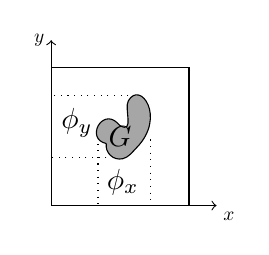
\begin{tikzpicture}[scale=0.35, every node/.style={transform shape}]
	\draw (0,0) -- ++(5,0) -- ++(0, 5) -- ++(-5,0) -- cycle;
	\draw [<->] (0,6) -- (0,0) -- (6,0);
	\node [below right, scale=2] at (6,0) {$x$};
	\node [left, scale=2] at (0,6) {$y$};
	
	\draw [fill=gray!70] (2,2.25) to [curve through={(2.4,3) .. (2.5,2.9) .. (2.8,3.8) .. (3.1,2.1) .. (2.6,1.7)}] (2,2.25);
	
	\node [scale=3] at (2.5,2.5) {$G$};
	\draw [dotted] (1.7,2.25) -- (1.7,0);
	\draw [dotted] (3.6,2.4) -- (3.6,0);
	
	\node[above, scale=3] at (2.6,0) {$\phi_x$};
	
	\draw [dotted] (2,1.75) -- (0,1.75);
	\draw [dotted] (2.8,4) -- (0,4);
	
	\node[right, scale=3] at (0,3) {$\phi_y$};
	\end{tikzpicture}
	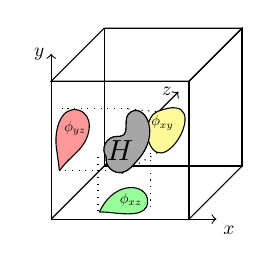
\begin{tikzpicture}[scale=0.35, every node/.style={transform shape}]
	\draw (0,0) -- ++(5,0) -- ++(0, 5) -- ++(-5,0) -- cycle;
	\draw (0,5,0) -- ++(0,0, -5) -- ++(5,0,0) -- ++(0,0,5) -- cycle;
	\draw (5,0,0) -- ++(0,0,-5) -- ++(0,5,0) -- ++(0,0,5) -- cycle;
	\draw (0,0,-5) -- ++(5,0,0) -- ++(0,5,0) -- ++(-5,0,0) -- cycle;
	\draw [<->] (0,6) -- (0,0) -- (6,0);
	\draw [->] (0,0,0) -- (0,0,-12);
	\node [left, scale=2, rotate=0] at (0,0,-12) {$z$};
	\node [below right, scale=2] at (6,0) {$x$};
	\node [left, scale=2] at (0,6) {$y$};
	
	\draw [fill=gray!70] (2,2.25) to [curve through={(2.4,3) .. (2.5,3) .. (2.8,3.8) .. (3.1,2.1) .. (2.6,1.7)}] (2,2.25);
	
	%				\node [scale=2] at (2.5,2.5) {$G$};
	\draw [dotted] (1.7,2.25) -- (1.7,0.2);
	\draw [dotted] (3.6,2.4) -- (3.6,0.3);
	
	\draw [fill=green!40] (1.75,0.25) to [curve through={(1.8, 0.35) .. (3.5, 0.65) .. (2,0.25)}] (1.75,0.25);
	\node[above, scale=1.5] at (2.6,0,-0.75) {$\phi_{xz}$};
	
	\draw [dotted] (2,1.75) -- (0.3,1.75);
	\draw [dotted] (2.8,4) -- (0.385,4);
	
	\draw [fill=red!40] (0.3, 1.75) to [curve through={(0.5,2) .. (1, 2.5) .. (1,3.95) .. (0.2, 2.5)}] (0.3,1.75);
	\node[right, scale=1.5] at (0,3, -0.75) {$\phi_{yz}$};
	
	\draw [fill=yellow!40] (3.85,3.9) to [curve through={(3.7,3.8) .. (3.5,3.4) .. (3.45,3.2)}] (3.85, 3.9);
	\node [scale=1.5] at (3.65,3.1,-1) {$\phi_{xy}$};
	\draw [dotted] (2.8,4) -- (3.8,3.9);
	\draw [dotted] (2.56,1.65) -- (4,2.5);
	
	\draw [fill=gray!70] (2,2.25) to [curve through={(2.4,3) .. (2.5,3) .. (2.8,3.8) .. (3.1,2.1) .. (2.6,1.7)}] (2,2.25);
	
	\node [scale=3] at (2.5,2.5) {$H$};
	\end{tikzpicture}
\end{center}
\vfill
\begin{itemize}
	\item Similarly, for a $4$d object $I$, $Volume(I) \le \phi_{xyz}^\frac13  \phi_{xyw}^\frac13 \phi_{xzw}^\frac13  \phi_{yzw}^\frac13$
	\vfill
	\item How to work with arbitrary dimensional projections?
\end{itemize}
	
\end{frame}

\begin{frame}{H\"{o}lder-Brascamp-Lieb (HBL) inequality}
	
	\small
	\begin{itemize}
		\item Generalize Loomis-Whitney inequality for arbitrary dimensional projections
		\vfill
		\item Provide exponent for each projection
\end{itemize}
\vfill
\begin{lemma}
	\label{lem:hbl}
	Consider any positive integers $\ell$ and $m$ and any $m$ projections $\phi_j:\mathbb{Z}^\ell\rightarrow\mathbb{Z}^{\ell_j}$ ($\ell_j\leq \ell$), each of which extracts $\ell_j$ coordinates $S_j\subseteq [\ell]$ and forgets the $\ell-\ell_j$ others.
	Define
%	$\mathcal{C} = \big\{\V{s}=[s_1\ \cdots \ s_m]^\Tra: 0\leq s_i \leq 1 \text{ for } i=1,2,\cdots,m \text{ and } \M{\Delta}\cdot\V{s}\ge\V{1}\big\}\text,$
	$\mathcal{C} = \big\{\V{s} \in[0,1]^m:\M{\Delta}\cdot\V{s}\ge\V{1}\big\}\text,$
	where the $\ell\times m$ matrix $\M{\Delta}$ has entries
	$\M{\Delta}_{i,j} = 1 \text{ if } i\in S_j \text{ and } \M{\Delta}_{i,j} = 0 \text{ otherwise}\text.$
	If $[s_1\ \cdots \ s_m]^\Tra\in\mathcal{C}$, then for all $F\subseteq \mathbb{Z}^\ell$,
	$$ |F| \leq \prod_{j\in [m]}|\phi_j(F)|^{s_j}\text.$$
\end{lemma}
\vfill
	\vspace*{-0.15cm}\begin{itemize}
	\item For tighter  bound, we usually work with $\M{\Delta}\cdot\V{s} = \V{1}$
	\begin{itemize}
		\item Possible that $\M{\Delta}\cdot\V{s} = \V{1}$ does not have solution, then consider $\V{s}$ such that $\M{\Delta}\cdot\V{s}$ is not very far from $\V{1}$
	\end{itemize}
\end{itemize}

\vfill
Notation: $\V{1}$ represents a vector of all ones. $[m]$ denotes $\{1, 2,\cdots, m\}$ throughout the slides.
\end{frame}

\begin{frame}{HBL inequality}
	\small
	
	\vspace*{-0.15cm}{\footnotesize\begin{lemma}
		\label{lem:hbl}
		Consider any positive integers $\ell$ and $m$ and any $m$ projections $\phi_j:\mathbb{Z}^\ell\rightarrow\mathbb{Z}^{\ell_j}$ ($\ell_j\leq \ell$), each of which extracts $\ell_j$ coordinates $S_j\subseteq [\ell]$ and forgets the $\ell-\ell_j$ others.
		Define
		%	$\mathcal{C} = \big\{\V{s}=[s_1\ \cdots \ s_m]^\Tra: 0\leq s_i \leq 1 \text{ for } i=1,2,\cdots,m \text{ and } \M{\Delta}\cdot\V{s}\ge\V{1}\big\}\text,$
		$\mathcal{C} = \big\{\V{s} \in[0,1]^m:\M{\Delta}\cdot\V{s}\ge\V{1}\big\}\text,$
		where the $\ell\times m$ matrix $\M{\Delta}$ has entries
		$\M{\Delta}_{i,j} = 1 \text{ if } i\in S_j \text{ and } \M{\Delta}_{i,j} = 0 \text{ otherwise}\text.$
		If $[s_1\ \cdots \ s_m]^\Tra\in\mathcal{C}$, then for all $F\subseteq \mathbb{Z}^\ell$,
		\vspace*{-0.15cm}$$ |F| \leq \prod_{j\in [m]}|\phi_j(F)|^{s_j}\text.$$
	\end{lemma}}
\vspace*{-0.15cm}
\begin{block}{Matrix multiplication ($C=AB$) example}
%		$C= AB$, where $A \in\mathbb{R}^{n_1 \times n_2}$, $B \in\mathbb{R}^{n_2 \times n_3}$, and  $C \in \mathbb{R}^{n_1 \times n_3}$.
		\vspace*{-0.25cm}\begin{columns}
			\begin{column}{0.6\linewidth}
				Here $A \in\mathbb{R}^{n_1 \times n_2}$, $B \in\mathbb{R}^{n_2 \times n_3}$, and  $C \in \mathbb{R}^{n_1 \times n_3}$.
					\vspace*{-0.15cm}\begin{align*}
				&\text{for $i = 1{:}n_1$, for $k = 1{:}n_2$, for $j = 1{:}n_3$}\\
				&\quad \quad C[i][j] += A[i][k]*B[k][j]
				\end{align*}
				\vfill
			\end{column}
			\begin{column}{0.35\linewidth}
					\begin{center}
					$\M{\Delta} = \begin{blockarray}{cccc}
					& A & B & C  \\
					\begin{block}{c(ccc)}
					i & 1 & 0 & 1\\
					j & 0 & 1 & 1\\
					k & 1 & 1 & 0\\
					\end{block}
					\end{blockarray}$
				\end{center}
			\end{column}\hfill
		\end{columns}
	\vspace*{-0.5cm}\begin{itemize}{
			\item Find $\V{s}=\begin{bmatrix} s_1 & s_2 & s_3 \end{bmatrix}^\Tra$ such that $\M{\Delta}\cdot\V{s} = \V{1}$
			\item $\phi_A, \phi_B, \phi_C$: projections of computations on arrays $A$, $B$, $C$
			\item HBL inequality:  $\text{Amount of computations} \le \phi_A^{s_1} \phi_B^{s_2} \phi_C^{s_3}$
%			\item To make inequality tight select $\V{x}$ such that $\V{1}^\Tra \V{x}$ is minimum $=>x_1=x_2=x_3 = \frac{1}{2}$ 
	}\end{itemize}\vspace*{-0.25cm}	
\end{block}
\end{frame}
\begin{frame}{HBL inequality}
	\small
	It an be used to obtain sequential or parallel communication lower bound.
	
	Sequential lower bound formulation for matrix multiplication:
	\begin{itemize}
		\item Determine maximum amount of computations under segment size constraint:  $Maximize\  \phi_A^{s_1} \phi_B^{s_2} \phi_C^{s_3}$ s.t.  $\phi_A + \phi_B + \phi_c <= Constt$
		\item Calculate total data transfers for all the segments
	\end{itemize}
\vfill
%We can work with $\M{\Delta}^\Tra$ to determine tile sizes of a sequential algorithm.
%\begin{itemize}
%	\item Find $\V{x}=\begin{bmatrix} x_1 & x_2 & x_3 \end{bmatrix}^\Tra$ such that $\M{\Delta}^\Tra\cdot\V{x} \le \V{1}$ and $\V{1}^\Tra x$ is maximum
%	\item $M^{x_i}$ is the tile dimension along $i$th axis
%	\item Usually results in asymptotic communication optimal algorithm.
%\end{itemize} 
%\vfill
	Parallel lower bound formulation for matrix multiplication:
	\begin{itemize}
		\item Determine the sum of array accesses to perform the required computations
		\begin{itemize}
			\item $Minimize\ \phi_A + \phi_B + \phi_c$  s.t. $\textnormal{amount of computations} \le \phi_A^{s_1} \phi_B^{s_2} \phi_C^{s_3}$
		\end{itemize}
	\end{itemize} 
\end{frame}
%	\usefonttheme[onlymath]{serif} 
\begin{frame}{Optimization problems [Ballard et al., IPDPS 2017]}
	\small
\footnotesize
%\begin{columns}
%	\begin{column}{0.475\linewidth}
%	\end{column}
%	\begin{column}{0.475\linewidth}
%	\end{column}
%\end{columns}
\vspace*{-0.15cm}\begin{lemma}
	Given $s_i >0$, the optimization problem 
	\vspace*{-0.15cm}$$\max_{x_i\ge 0} \prod_{i\in[m]} x_i^{s_i} \textnormal{ subject to } \sum_{i\in [m]} x_i \le c$$
	yields the maximum value
	\vspace*{-0.15cm}$$c^{\sum_i s_i}\prod_{j\in [m]} \left(\frac{s_j}{\sum_i s_i}\right)^{s_j}\text.$$
\end{lemma}
\vfill
\vspace*{-0.15cm}\begin{lemma}
	Given $s_i >0$, the optimization problem 
	\vspace*{-0.15cm}$$\min_{x_i\ge 0} \sum_{i\in [m]} x_i  \textnormal{ subject to }  \prod_{i\in[m]} x_i^{s_i} \ge  c$$
	yields the maximum value
	\vspace*{-0.15cm}$$\left(\frac{c}{\prod_i {s_i}^{s_i}}\right)^\frac{1}{\sum_i s_i} \sum_{j\in[m]} s_j\text.$$
\end{lemma}
\vfill
Both lemmas can be proved with the Lagrange multipliers.
\end{frame}
\section{CP decomposition}
	\begin{frame}{Table of Contents}		
	\tableofcontents[currentsection,hideallsubsections] % Output the table of contents (all sections on one slide)		
\end{frame}
\begin{frame}{CP decomposition of $\T{A} \in \mathbb{R}^{n_1\times n_2\times\cdots\times n_d}$}
	\small
	It factorizes a tensor into a sum of rank one tensors.
	\begin{center}
		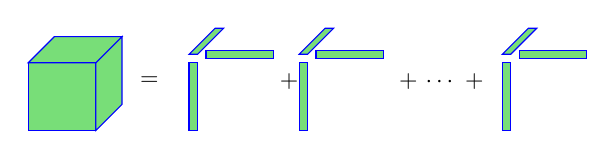
\begin{tikzpicture}[scale=0.215, every node/.style={transform shape}]
		\pgfmathsetmacro{\cubex}{4}
		\pgfmathsetmacro{\cubey}{4}
		\pgfmathsetmacro{\cubez}{4}
		\draw[blue,fill=pastelgreen] (0,0,0) -- ++(-\cubex,0,0) -- ++(0,-\cubey,0) -- ++(\cubex,0,0) -- cycle;
		\draw[blue,fill=pastelgreen] (0,0,0) -- ++(0,0,-\cubez) -- ++(0,-\cubey,0) -- ++(0,0,\cubez) -- cycle;
		\draw[blue,fill=pastelgreen] (0,0,0) -- ++(-\cubex,0,0) -- ++(0,0,-\cubez) -- ++(\cubex,0,0) -- cycle;
		
		\node[draw=none, text=black, scale=4] at (2,-2.25,-3) {$=$};
		\pgfmathsetmacro{\smallwidth}{0.5}
		\draw[blue,fill=pastelgreen] (\cubex+2,0,0) -- ++(-\smallwidth,0,0) -- ++(0,-\cubey,0) -- ++(\smallwidth,0,0) -- cycle;
		\draw[blue,fill=pastelgreen] (\cubex+2 +\cubex + 0.5,0.75,0) -- ++(-\cubex,0,0) -- ++(0,-\smallwidth,0) -- ++(\cubex,0,0) -- cycle;
		\draw[blue,fill=pastelgreen] (\cubex+2,0.5,0) -- ++(-\smallwidth,0,0) -- ++(0,0,-\cubez) -- ++(\smallwidth,0,0) -- cycle;
		
		\node[draw=none, text=black, scale=4] at (2+\cubex+4.25,-2.25,-3) {$+$};
		
		\draw[blue,fill=pastelgreen] (\cubex+2.5 + \cubex+2,0,0) -- ++(-\smallwidth,0,0) -- ++(0,-\cubey,0) -- ++(\smallwidth,0,0) -- cycle;
		\draw[blue,fill=pastelgreen] (\cubex+2.5+\cubex+2 +\cubex + 0.5,0.75,0) -- ++(-\cubex,0,0) -- ++(0,-\smallwidth,0) -- ++(\cubex,0,0) -- cycle;
		\draw[blue,fill=pastelgreen] (\cubex+2.5+\cubex+2,0.5,0) -- ++(-\smallwidth,0,0) -- ++(0,0,-\cubez) -- ++(\smallwidth,0,0) -- cycle;
		
		\node[draw=none, text=black, scale=4] at (2+\cubex+5 + \cubex+ 4.25, -2.25,-3) {$+$ $\cdots$ $+$};
		
		\draw[blue,fill=pastelgreen] (12 + \cubex+2.5 + \cubex+2,0,0) -- ++(-\smallwidth,0,0) -- ++(0,-\cubey,0) -- ++(\smallwidth,0,0) -- cycle;
		\draw[blue,fill=pastelgreen] (12+\cubex+2.5+\cubex+2 +\cubex + 0.5,0.75,0) -- ++(-\cubex,0,0) -- ++(0,-\smallwidth,0) -- ++(\cubex,0,0) -- cycle;
		\draw[blue,fill=pastelgreen] (12 + \cubex+2.5+\cubex+2,0.5,0) -- ++(-\smallwidth,0,0) -- ++(0,0,-\cubez) -- ++(\smallwidth,0,0) -- cycle;
		\end{tikzpicture}
	\end{center}
	\vspace*{-0.15cm}\centering{\footnotesize CP decomposition of a $3$-dimensional tensor.}
	\vfill
	{\footnotesize\vspace*{-0.1cm}$$\T{A}=\sum_{\alpha=1}^{r} U_1 (:,\alpha) \circ U_2(:,\alpha)\circ\cdots \circ U_d(:,\alpha)$$}
	%		$$\T{A}(i_1,\cdots,i_d) = \sum_{\alpha=1}^{r} U_1(i_1,\alpha) U_2(i_2,\alpha)\cdots U_d(i_d,\alpha)$$}
	\vfill
	\justifying
	It can be concisely expressed as $\T{A} = \llbracket U_1, U_2, \cdots, U_d \rrbracket$. CP decomposition for a $3$-dimensional tensor in matricized form can be written as:
	$$A_{(1)}=U_1(U_3\odot U_2)^T,\ A_{(2)}=U_2(U_3\odot U_1)^T\ A_{(3)}=U_3(U_2\odot U_1)^T\text.$$
	
	\vfill
	It is useful to assume that $U_1, U_2 \cdots U_d$ are normalized to length one with the weights given in a vector $\lambda \in \mathbb{R}^r$.
	
\end{frame}

\begin{frame}{CP-ALS algorithm for a 3-dimensional tensor $\T{A}$}
	\small
	\textbf{Repeat} until maximum iterations reached or no further improvement obtained
	\begin{enumerate}
		\item Solve $U_1(U_3\odot U_2)^T = A_{(1)}$ for $U_1$ $\Rightarrow U_1 = A_{(1)} (U_3\odot U_2) (U_3^TU_3 * U_2^TU_2)^\dagger$
		\item Normalize columns of $U_1$
		\item Solve $U_2(U_3\odot U_1)^T = A_{(2)}$ for $U_2$ $\Rightarrow U_2 = A_{(2)} (U_3\odot U_1) (U_3^TU_3 * U_1^TU_1)^\dagger$
		\item Normalize columns of $U_2$
		\item Solve $U_3(U_2\odot U_1)^T = A_{(3)}$ for $U_3$ $\Rightarrow U_3 = A_{(3)} (U_2\odot U_1) (U_2^TU_2 * U_1^TU_1)^\dagger$
		\item Normalize columns of $U_3$
	\end{enumerate}
	
	\bigskip
	Here $A^\dagger$ denotes the Moore--Penrose pseudoinverse of $A$. We use the following identity to get expressions for $U_1, U_2$ and $U_3$:
	$$(A\odot B)^T(A\odot B) = A^TA * B^TB$$
\end{frame}
\begin{frame}{ALS for computing a CP decomposition}
	\small
	\vspace*{-0.25cm}\begin{algorithm}[H]{
			\caption{CP-ALS method to compute CP decomposition\label{alg:canonicalals}}
			%%				\caption{HOSVD Algorithm($\X$, $R_1$, $R_2$, $R_3$)}
			\begin{algorithmic}
				\Require input tensor $\T{A}\in \mathbb{R}^{n_1\times \cdots \times n_d}$, desired rank $k$, initial factor matrices $U_j\in \mathbb{R}^{n_j\times k} \textnormal{ for } 1\le j \le d$
				\Ensure $\llbracket \lambda; U_1, \cdots, U_d\rrbracket $ : a rank-$k$ CP decomposition of $\T{A}$
				\Repeat
				\For{$i=1 \text{ to } d$}
				\State $V\gets U_1^\Tra U_1*\cdots*U_{i-1}^\Tra U_{i-1} U_{i+1}^\Tra U_{i+1} *\cdots*U_d^\Tra U_d$
				\State $U_i \gets A_{(i)} (U_d\odot\cdots\odot U_{i+1}\odot U_{i-1}\odot U_1)$\label{alg:canonicalals:mttkrp}
				\State $U_i\gets U_iV^\dagger$ 
				\State $\lambda\gets \text{normalize colums of } U_i$ 
				\EndFor
				\Until converge or the maximum number of iterations
			\end{algorithmic}
	}\end{algorithm}
%	\vspace*{-0.375cm}
	\begin{itemize}
		\item The collective operation $A_{(i)} (U_d\odot\cdots\odot U_{i+1}\odot U_{i-1}\odot U_1)$ is known as Matricized tensor times Khatri-Rao product (MTTKRP) computation
%		\item $U_j$ can be chosen randomly or by setting $k$ left singular vectors of $A_{(j)}$ for $1\le j \le d$
	\end{itemize}	
\end{frame}

\end{document} 